\documentclass[12pt]{article}

\usepackage{verbatim}
\usepackage{listings}
\usepackage{color}
\usepackage{graphicx}
\usepackage{amsmath}


%%
\title{H bridge basics}

\author{Fabien Le Mentec\\
\small \texttt{texane@gmail.com}
}

\date{}

\begin{document}
\maketitle

\begin{abstract}
This document describes the basics of H bridges. The primary goal is to learn more about electronics.
\end{abstract}


%% Introduction
\newpage
\section{Introduction}

\subsection{Purpose}
\paragraph{} I wanted a small project to learn more about electronics basics. Since I regularly need to
drive a DC motors, I chose to work on a home made H bridge board described in this document. Note that
the circuit uses off the shelf parts and can be more complicated than needed and not efficient. A real
application should use packaged H bridge circuits.


%% Features
\newpage
\section{Features}
\paragraph{} The board features:
\begin{itemize}
  \item 3 wires, safe H signaling interface, avoiding invalid transistor states
    \begin{itemize}
      \item PWM,
      \item FORWARD,
      \item BRAKE.
    \end{itemize}
  \item controlling software
    \begin{itemize}
      \item coding done by XXX
    \end{itemize}
  \item power stage driving up to XXX motors.
\end{itemize}


%% Theory of operation
\newpage
\section{H bridge theory of operation}
\paragraph{} An H bridge is a circuit allowing to drive DC motors in both direction. The name comes from the
typical circuit graphical representation which looks like the 'H' alphabet letter.

\begin{center}
  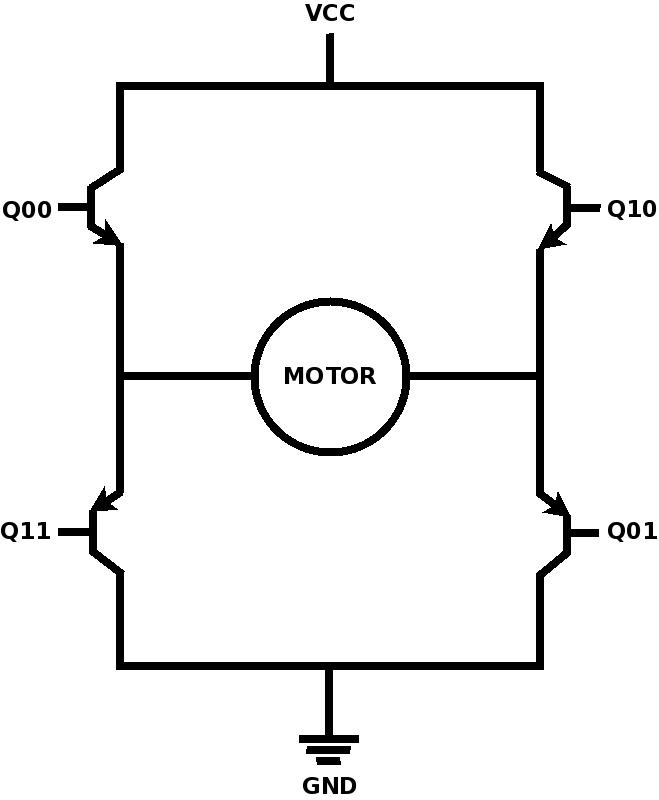
\includegraphics[keepaspectratio=true, width=40mm]{../pics/hbridge_base.jpg}
  \\
  \smallskip
  \tiny{\textit{H bridge circuit}}
\end{center}

QXX are transistors allowing the current flowing through the DC motor to be electrically controlled. I am
interested in 3 configurations:

\begin{center}
  \begin{tabular}{c|c|c}
    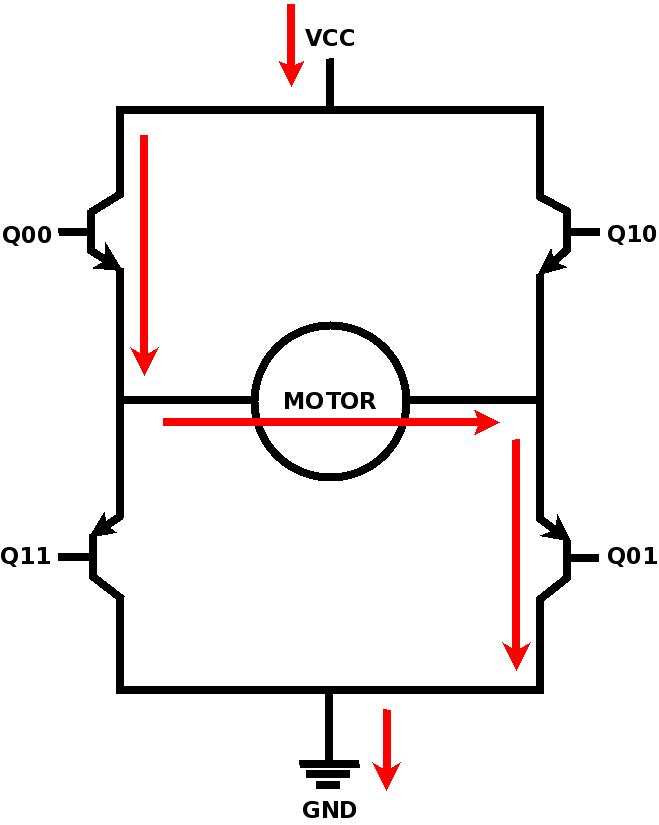
\includegraphics[keepaspectratio=true, width=40mm]{../pics/hbridge_forward.jpg} &
    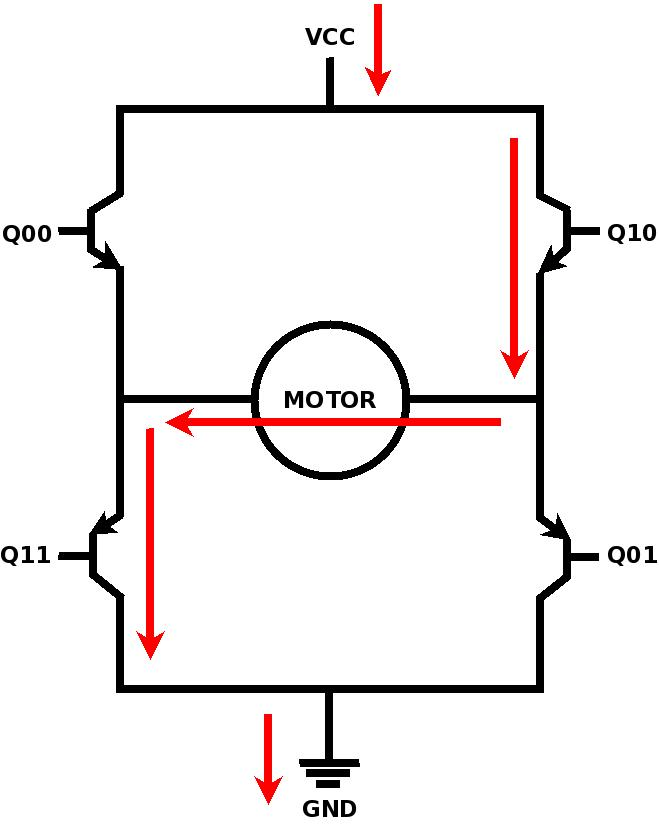
\includegraphics[keepaspectratio=true, width=40mm]{../pics/hbridge_reverse.jpg} &
    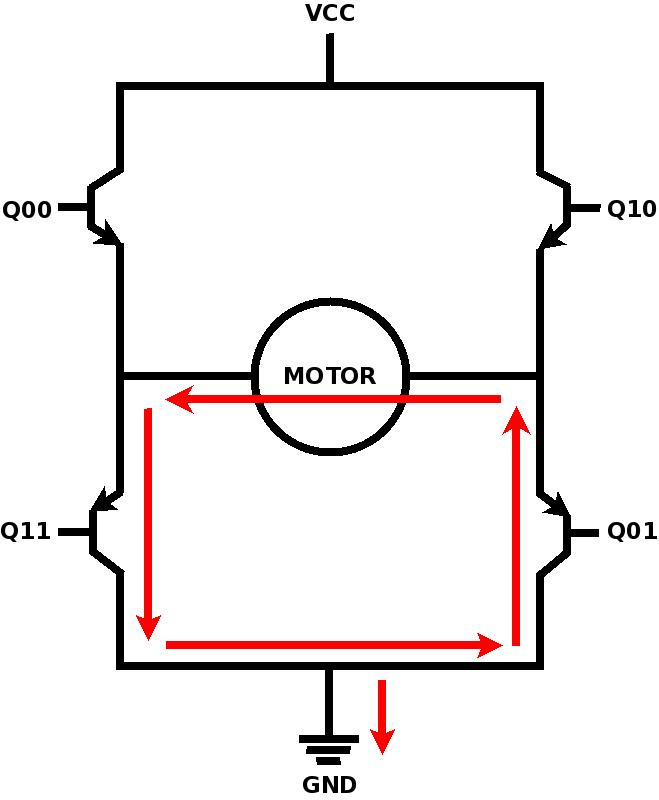
\includegraphics[keepaspectratio=true, width=40mm]{../pics/hbridge_brake.jpg} \\
    \tiny{\textit{FORWARD mode}} & \tiny{\textit{REVERSE mode}} & \tiny{\textit{BRAKE mode}}
  \end{tabular}
\end{center}

%% H signaling interface
\newpage
\section{H signaling interface}

\paragraph{} The H bridge expects a correct transistor configuration to work. Even worth, an incorrect setup can
damage the circuit and motor. I designed a 3 wire signaling interface, called the H signaling interface, to address
this issue:

\smallskip
\begin{center}
  \begin{tabular}{|c|c|}
    \hline
    \textit{Name} & \textit{Description} \\
    \hline
    FWD & controls the motor direction \\
    \hline
    PWM & controls the motor speed \\
    \hline
    BRAKE & slow the motor down until it stops \\
    \hline
  \end{tabular}
  \\
  \smallskip
  \tiny{\textit{H control signals}}
\end{center}

\paragraph{} Since I have a software background it is easier for me to think in terms of C programming control
structures. I thus express the H state machine in a C code which I then translate into logical statements. I
use the resulting statement set to design the H state circuit using electronic gates.

\smallskip
\begin{tiny}
  \lstset{commentstyle=\color{blue}}
  \lstset{language=C}
  \begin{lstlisting}[frame=tb]
if (BRAKE == 0)
{
  if (FWD == 1)
  {
    Q01 = 0;
    Q10 = 0;
    Q11 = 1;

    Q00 = PWM;
  }
  else /* REVERSE */
  {
    Q00 = 0;
    Q01 = 1;
    Q11 = 0;

    Q10 = PWM;
  }
}
else /* (BRAKE == 1) */
{
  Q00 = 1;
  Q01 = 1;
  Q10 = 1;
  Q11 = 1;
}
  \end{lstlisting}
\end{tiny}

\smallskip
The above code reduces to the following set of logical statments:
\begin{tiny}
  \lstset{commentstyle=\color{blue}}
  \lstset{language=C}
  \begin{lstlisting}[frame=tb]
Q00 = (FWD & PWM)    | BRAKE;
Q01 = (!FWD)         | BRAKE;
Q10 = ((!FWD) & PWM) | BRAKE;
Q11 = FWD            | BRAKE;
  \end{lstlisting}
\end{tiny}

\smallskip
\pagebreak
These 4 statements are implemented by the following circuit:
\begin{center}
  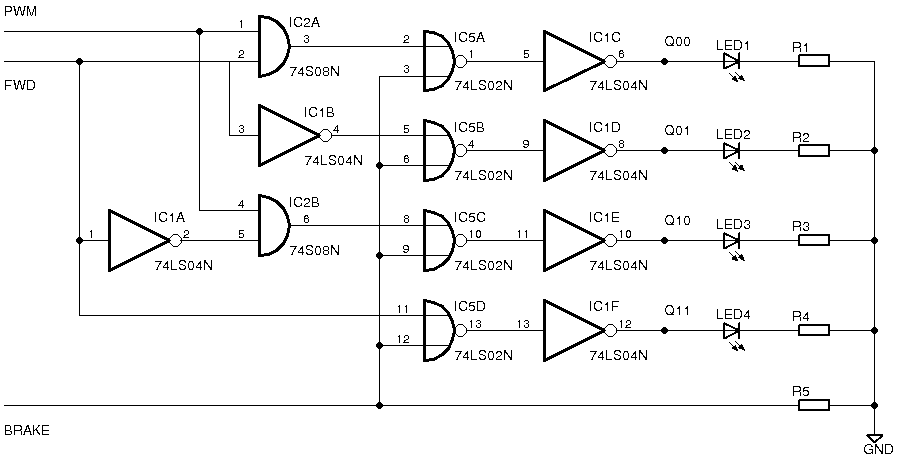
\includegraphics[keepaspectratio=true, width=1.\textwidth]{../pics/h_control.png}
  \\
  \smallskip
  \tiny{\textit{H control circuit}}
\end{center}

Note that I do not have OR gates, so I used NOR gates and inverters. It complexifies the circuit a bit.
Apart from that, the logical statements are naively implemented using electronic gates.

\smallskip
\begin{center}
  \begin{tabular}{|c|c|c|}
    \hline
    \textit{Reference} & \textit{Quantity} & \textit{Description} \\
    \hline
    SN74LS02N & 1 & quad 2 input NOR gates \\
    \hline
    SN74LS04N & 1 & hex inverter \\
    \hline
    SN74LS08N & 1 & quad 2 input AND gates \\
    \hline
    Resistors & 5 & 2.4k ohms \\
    \hline
    LEDS & 4 & \\
    \hline
  \end{tabular}
  \\
  \smallskip
  \tiny{\textit{part list}}
\end{center}

\smallskip
\pagebreak
Picture of the prototyped circuit, with switchs added for testing:
\begin{center}
  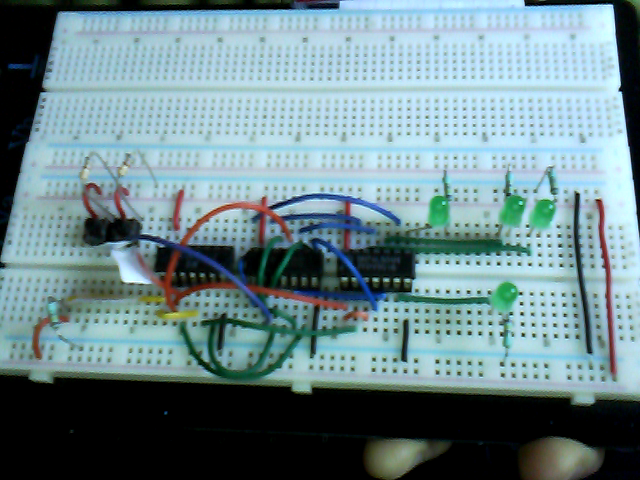
\includegraphics[keepaspectratio=true, width=1.\textwidth]{../pics/h_control_breadboard.png}
  \\
  \smallskip
  \tiny{\textit{H control circuit prototype}}
\end{center}


%% H bridge transistors
\newpage
\section{H bridge transistors}

\begin{center}
  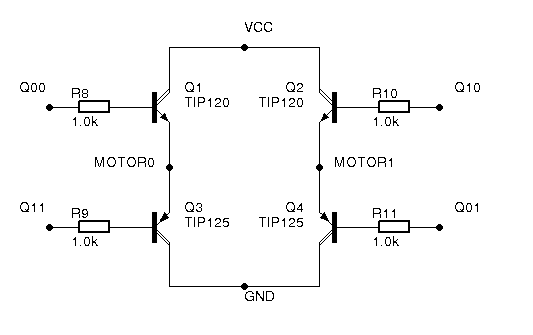
\includegraphics[keepaspectratio=true, width=100mm]{../pics/h_transistors.png}
  \\
  \smallskip
  \tiny{\textit{H bridge transistors}}
\end{center}

\smallskip
\begin{center}
  \begin{tabular}{|c|c|c|}
    \hline
    \textit{Reference} & \textit{Quantity} & \textit{Description} \\
    \hline
    TIP120 & 2 & complementary power darlington transistors \\
    \hline
    TIP125 & 2 & complementary power darlington transistors \\
    \hline
    Resistors & 4 &  1.0k \\
    \hline
  \end{tabular}
  \\
  \smallskip
  \tiny{\textit{part list}}
\end{center}


%% H controlling logic
\newpage
\section{PWM generation}
IN PROGRESS

\subsection{PWM basics}
The motor speed is controlled using a PWM signal.\\
TODO: explain duty cycle, averaged total current as a function of time

\subsection{PWM using transistors}
TODO

\subsection{PWM using a NE555}
\paragraph{} I use a NE555 chip in an astable setup to generate a PWM signal. The Philips 555
application note has been used as a reference for this section. The circuit is shown below:
\begin{center}
  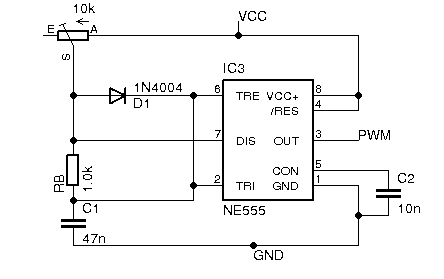
\includegraphics[keepaspectratio=true, width=1.\textwidth]{../pics/ne555_astable.png}
  \\
  \smallskip
  \tiny{\textit{NE555 astable setup}}
\end{center}

\begin{center}
  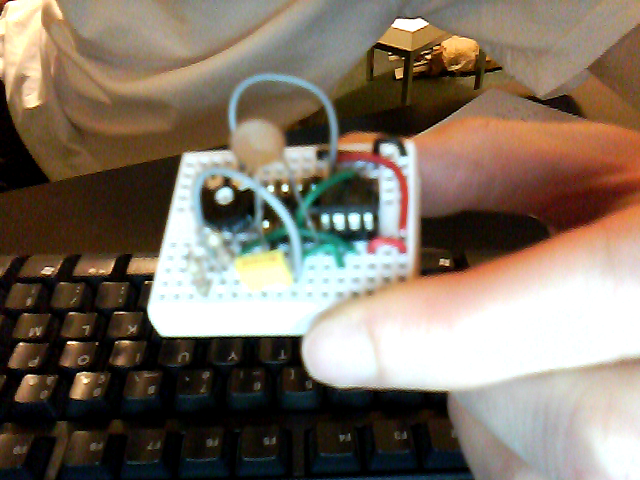
\includegraphics[keepaspectratio=true, width=60mm]{../pics/ne555_astable_circuit.png}
  \\
  \smallskip
  \tiny{\textit{NE555 astable circuit}}
\end{center}

2 things to note:
\begin{itemize}
\item a pot is use to control the duty cycle by varying the voltage divider ratio,
\item a diode between pins 6 and 7 has been added to allow a duty of less than 50\%.
\end{itemize}

The documentation gives the following formula:
\begin{center}
\framebox[3in][c]{$ Frequency = \frac{1.49}{((Ra + 2 * Rb) * C1)} $}
\end{center}

In the above circuit, the following values are used:
\begin{itemize}
\item Ra = 0 to 10k,
\item Rb = 1k,
\item C1 = 47n.
\end{itemize}

By substitution, we have:
\begin{center}
\framebox[4.5in][c]{$ \frac{1.49}{(2 * 10^3 + 10 * 10^4) * 47 * 10^-9} <= frequency <= \frac{1.49}{2 * 10^3 * 47 * 10^-9} $}
\end{center}

Thus:
\begin{center}
\framebox[3in][c]{$ 2642 <= frequency <= 15851 $}
\end{center}

\begin{itemize}
\item TODO: old result from a different configuration
\item TODO: picture of the oscilloscope screen
\end{itemize}
The frequencies can be checked using an oscilloscope:
\begin{center}
\framebox[3in][c]{$ 2272 <= frequency <= 10000 $}
\end{center}

\subsection{PWM using an AVR microcontroller}
TODO

%% H controlling software
\newpage
\section{H controlling software}
TODO


%% Status
\newpage
\section{Status}
\begin{itemize}
  \item PWM / FORWARD / BRAKE signaling interface: PROTOTYPED
  \item control software: TODO
  \item transistor stage: PROTOTYPED
  \item documentation: INPROGRESS
\end{itemize}


%% Conclusion
\newpage
\section{Conclusion}
\begin{center}
  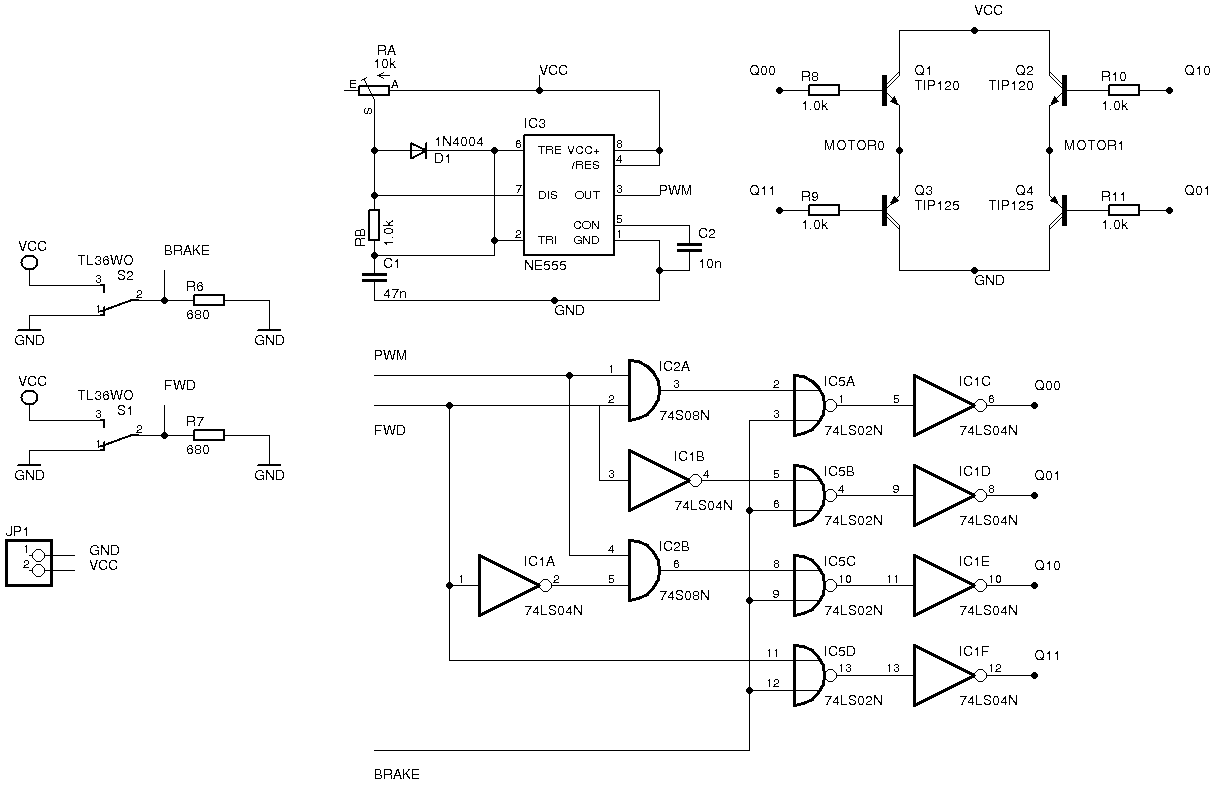
\includegraphics[keepaspectratio=true, scale=0.86]{../pics/h_full.png}
  \\
  \smallskip
  \tiny{\textit{full H bridge circuit}}
\end{center}


%% References
\newpage
\section{Further readings}

\subsection{H bridge projects}
\begin{itemize}
  \item http://embedded-lab.com/blog/?p=1159
  \item http://www.mcmanis.com/chuck/robotics/tutorial/h-bridge
  \item http://www.modularcircuits.com/h-bridge\_secrets1.htm
  \item http://www.solarbotics.net/library/circuits/driver\_4varHbridge.html
  \item http://www.solarbotics.net/library/circuits/driver\_buf\_h.html
  \item http://www.robotroom.com/HBridge.html
  \item http://www.robotroom.com/BipolarHBridge.html
  \item http://www.societyofrobots.com/schematics\_h-bridgedes.shtml
\end{itemize}

\subsection{Controlling software}
\begin{itemize}
  \item http://www.seattlerobotics.org/encoder/200001/simplemotor.htm
\end{itemize}


%% TODO
\section{TODO}

\begin{itemize}
\item PWM using ne555
\begin{itemize}
  \item oscilloscope pictures
  \item wider duty cycle range
  \item how to compute the duty range
  \item more about the 555
\end{itemize}
\item Atmel AVR or ne555 or RC network + variable resistor to control motor speed
\item controlling software 
\end{itemize}


\end{document}
